
% \setcounter{chapter}{2}
\newchapter{Evidence of Strategic Social Learning and Evolutionary Arms Races in the Opening Moves of the Game of Go}{Evidence of Strategic Social Learning and Evolutionary Arms Races in the Opening Moves of the Game of Go}{Evidence of Strategic Social Learning and Evolutionary Arms Races in the Opening Moves of the Game of Go}

\section{Introduction}

% intro should be addressed towards the committee...we can revise once it's accepted as phd chapter

One of the greatest contributions of evolutionary theory is the ability to answer ``why'' questions about living things, explaining the existence of their intricate and beautiful designs as adaptations via natural selection.  This success extends to study of our own species; we now know a great deal about our behavior, psychology and, more indirectly, our ancestry, as a consequence of evolutionary theory \citep{LalandBrown2002sense, Barkow1992adaptedmind}.  Many pathological or idiosyncratic human social phenomena, for example, can be understood via the ``mismatch'' hypothesis, whereby our minds and bodies are ``expecting'' one particular environment (subsistence foraging) yet placed in another (industrial food markets and sedentary lifestyles).  

This evolutionary research program has revolutionized the study of human beings, and greatly aids our understanding of human thought and behavior.  It is less clear, though, how ancestral psychological adaptations can explain the dynamics of human history.  Such research must necessarily involve the evolution of technology and other forms of culture, and how these inherited artifacts, institutions and ideas structure human cognition and decision-making at particular times and places.  

Work in the last three decades has approached this problem by recognizing culture is a system of inheritance, akin to genes \citep{Richerson2005:NBGA, durham1992coevolution}.  Mathematical models have shown that such a system necessarily exhibits Darwinian adaptive dynamics, even if the traits under study are not discrete, particulate replicators like genes, and even if they are not created at random as in genetic mutation \citep{boyd1985culture, Henrich2002}  Thus, by applying what Ernst Mayr called ``population-thinking'' to human culture, we can see how socially-transmitted technologies, beliefs and behaviors spread and decline over time because of the quotidian events in the lives of their human users \citep{Shennan2009, Mesoudi2006}.

As with genetic evolution, these processes can be organized within a set of general categories we call ``forces'', but unlike natural selection, genetic drift, meiotic drive, etc., the forces of cultural evolution are largely based on the nature of human psychology.  What humans find easy or appealing to learn, what cues and associations they find salient, and how readily certain cultural traits encourage their own social transmission all help drive the spread of particular technologies, beliefs and behaviors, and, as a result, much research in cultural evolution has concentrated on their study \citep{Richerson2005:NBGA}. 

A staple of this work has been laboratory and field experiments in which participants are given controlled access to potentially valuable social information \citep{caldwell2008studying, baum2004cultural, Mesoudi2011a, effersontakezawa2007}.  These projects have shown that simple social learning heuristics, such as ``when in doubt, copy what the majority is doing'' are quite plausible explanations for how humans learn from others.  However, there remains a great need for long-term, non-experimental datasets that have sufficient detail to tell us if such learning behaviors plausibly drive real-world cultural dynamics.  

Studying cultural evolution in such historical contexts is much harder task.  When cautious, observational research struggles to identify the importance of different underlying evolutionary mechanisms.  Michel et al. \citeyearpar{michel2011quantitative} use Google book archives to trace word use frequencies over the last several centuries but, lacking information about \textit{who} is using those words, are unable to explain these trends beyond phenomenological descriptions and qualitative associations to historical events.  A clever approach by Henrich \citeyearpar{Henrich2001} is to compare the common sinusoidal curve of technological diffusions to the predicted shapes emerging from a variety of individual-level learning models.  Ideally, we could go further in detecting particular evolutionary mechanisms if we knew who held a particular belief or practiced a behavior, what social ties connected individuals together, and could track this population over many years.  This is, of course, exactly analogous to the big-data demographic work in evolutionary demography \citep{grant2002unpredictable, ozgul2009dynamics}.  

In what follows, we present an analysis of one exceptionally high-resolution record of cultural patterns: historical game records from the East Asian game of Go.  Though a modest foray into a rich historical archive, our results provide strong evidence that, on the average, professional Go players use the social knowledge available for a particular game move - its prevelance and performance - to decide whether or not to use it in their own games.  This learning process, in aggregate, is thus largely responsible for driving population trends in Go openings among professional players.

Our argument proceeds as follows: first, we describe the nature of the study system, and establish that while the game of Go is enormously complex, professional players follow a narrow set of norms governing opening play that allows us to keep track of only a few common move variants.  We establish some gross historic patterns of these opening sequences, and focus in particular on the very first move in 20th century play, and the rise of the ``Fourfour'' variant.  

Second, using player-level data, we use the method of evolutionary decomposition (Beheim \& Baldini, in press) show that the prevalence of the Fourfour variant can only be explained by some form of learning, as opposed to demographic replacement or cohort effects.  Having established the importance of player decision-making, we then construct a variety of predictive models that take into account social and individual information and compare them using information-theoretic methods.  From these, we can determine that the interaction between the Fourfour's popularity and performance among the professional Go community is an excellent predictor of individual use, even after accounting for a player's personal experiences with the move.

Finally, knowing the predictive importance of social knowledge, we focus our attention on the strategic environment of the late 1960s and 1970s.  The database shows that the rise of the Fourfour opening move set off a period of counter-innovation in which new, more effective responses were developed.  Because of the resolution of the data, we can trace these innovations to particular players, and indeed particular games in which they first appeared.  


\section{Professional Go}

The East Asian board game known in the West as Go is, by players, one of the most popular games in the world, and certainly one of the oldest living games.  Originating in China between two and three thousand years ago (where it is called \textit{weiqi}), it has since diffused to Korea (there the game is called \textit{baduk}) and Japan (\textit{igo} or \textit{go}).  Through the Japanese, it became widely known in the West in the early 20th century, and most American and European Go terminology is derived from the Japanese ones.

The rules of the game are easily explained: there are two players, ``Black'' and ``White'', named after the colors of their uniform, button-shaped stones, who sit on opposite sides of a large 19x19 coordinate grid.  Starting with Black, each player takes turns placing a single stone on an empty grid intersection of their choice, until they agree to stop.  At the end of the game, the player who controls the majority of the board (that is, whose stones surround or occupy the most grid intersections) is the winner.  If the eventual outcome is obvious, one player may resign mid-game; otherwise, once all possible moves have been played, the players count grid intersections to see who is the winner.
 
Beyond this basic outline of the game, there are two key rules regulating play.  First, stones or groups of stones of one player that become completely surrounded in all four cardinal directions by stones of the other are removed from the board (this is the only time stones are moved, once placed).  Second, to prevent the possibility of the game entering an infinite loop, the \textit{ko} rule restricts play so that the same board state cannot appear twice in one game.

Though the rules above are remarkably simple, the game is fantastically complex, and it takes years of dedicated study to become a competitive player.  Much of one's skill in Go comes from the ability to make judgements about the long-term influence of particular moves and formations on the board, a task that currently bedevils attempts at developing competent artifical opponents \citep{Rimmel2010}.

Historically, the game was supported by the Tokugawa regime in Japan, which sponsored four competing houses.  Today, public enthusiasm in print and television broadcasts of games in East Asia funds several professional organizations, which employ full-time players who compete in national and international matches.  Entry into the professional leagues in Japan, China and Korea is extremely difficult, and top players usually begin serious study in adolescence.  Professional players are incredibly skilled and can easily defeat strong amateurs in even games.  Currently, the best professional players outmatch any computer program, even with a large handicap.  


\begin{figure}[t]
\begin{center} 
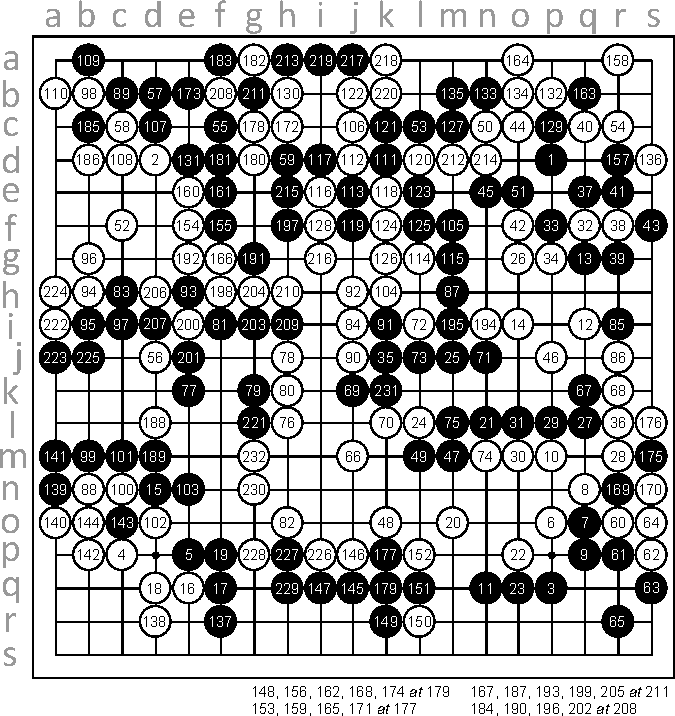
\includegraphics[scale=0.8]{figures/gofirstmove/figKifu.pdf}
\caption{A complete game record, with SGF coordinates, for a 1978 game between Japanese professionals Takemiya Masaki and Kudo Norio.  White (Kudo) won by resignation after 232 moves.  This match has significance in the opening move innovation race, as described in Section \ref{sec:Arms}.}
\label{fig:Kifu}
\end{center}
\end{figure}
 
Go games are quite easy to record, requiring only a single picture of the board at the end of the game, annotated with the sequence of moves played and notes for any stones that were removed (e.g. Figure \ref{fig:Kifu}).  Game records from top players and important tournaments have appeared in Japanese newspapers since the turn of the 20th century, often with professional commentary, and are now regularly published online as well.  In addition, many books of problems and strategies are avaliable in East Asia, usually written by active or retired professional players.  Topics in the Go literature range from analysis of specific moves or tactics to broader strategic ideas about play.  One common feature of studying the game is learning proverbs, which impart general lessons about good and bad play in a simple heuristic fashion \footnote{Examples from Segoe Kensaku's \textit{Go Proverbs Illustrated} \citeyearpar{Segoe1960} include ``When your opponent has two weak groups, attack them both at once.'' and ``One point in the center is worth ten in the corner.''}

Digital records of game records have become standardized using the SGF (``Smart Game Format'') markup to document move sequences and metadata in plaintext files.  Though large archives of professional games, stretching back centuries, exist in East Asia, only a fraction have been digitized.  In recent years, tens of thousands of amateur games are played each year on the internet, many of which are freely available in massive online SGF repositories.    

Two British Go historians, John Fairbairn and T Mark Hall, maintain a commercially available SGF database of professional games (``Games of Go on Disk'', or GoGoD) stretching back centuries.  Fairbairn and Hall have conducted extensive commentary and analyses of their database and have made their results freely available online.  One anecdote from their papers is quite telling: for a particular opening pattern\footnote{In SGF notation, \texttt{B[pd]W[dp]B[pp]W[dd]B[pj]W[nc]B[pf]W[jd]}; a less common variant pattern switches Move 2 and Move 4.}, master 20th century player Go Seigen\footnote{Japanese player names throughout this paper are written surname first, followed by given name.} remarked in a 1996 interview that the eighth move by White at SGF board coordinate jd was poor.  Fairbairn and Hall report that 

\begin{quote}
...a database search revealed, in over 120 games, that just about every top pro had played White 8 in this position. Indeed, the very first to do so was... Go Seigen (in 1936). More alarmingly, White had a whopping 56\% winning rate - that is unusually large...[however] when Go made this comment...around 1996, virtually all pros suddenly stopped playing White [at this position]. \citep{Fairbairn2009}
\end{quote}

Such descriptions are tantalizing evidence that professional Go game records contain clear evidence of the social learning dynamics thought to drive much of cultural evolution.  The international professional community is small enough for information to spread quickly from person to person, and most (nearly 90\%) professional players can be connected by one or two links in a match network in the GoGoD database.  Indeed, we assert that the essential features of professional Go - wide-open strategy space, clear performance measures, cumulative innovation, steep learning curve, pervasive norms of action, large community of players, and strong financial and social incentives for success - make it an ideal model system for studying how culture evolves in its broadest sense.  

To that end, we have developed software in the \texttt{R} computing language to aid in the analysis of SGF game archives (the \texttt{kaya} package).  In this analysis, we limit ourselves to 34,251 professional games drawn from the GoGoD archive, spanning the years 1956 to 2009.  Because our focus here is on the behavior of players over their careers, we excluded players with fewer than 50 games on record for Black, leaving 207 unique players.

\subsection{Historical Patterns of Opening Play}

Throughout a game of Go, the players can place their stones at virtually any open grid intersection.  Yet almost all competitive games follow the same basic pattern: initially, Black and White play in the four corners of the board, a few grid lines away from the board's edge (Figure \ref{fig:Heat}).  Play continues along the corners and sides until after the first 50 moves, at which time the players focus on the center of the board, for the main battles of the game.  About 42\% of games in the database end before Move 200, but if they continue, the average focus of play moves towards the outer edge of the board where the last few points of territory are claimed.  

Despite having the maximum number of possibilities, the first few moves of the game are actually the most predictable.  The opening period of the game is often characterized by highly normative, canalized play, where Black and White often follow one of a set of memorized move sequences called \textit{joseki} (or \textit{jungsuk} in Korea), thought to grant neither player a major advantage.  As with Chess openings, strong players maintain an encyclopedic knowledge of explored routes once a particular \textit{joseki} pattern has started.  


\begin{figure}[t]
\begin{center} 
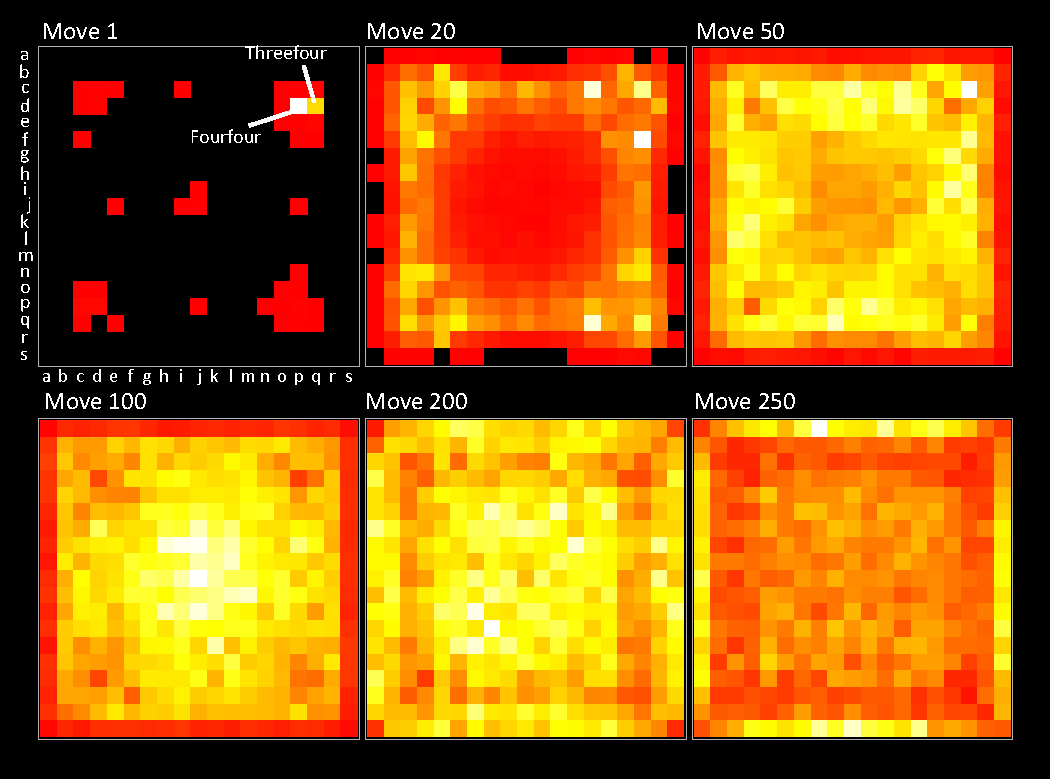
\includegraphics[scale=0.6]{figures/gofirstmove/figHeat.pdf}
\caption{Distribution of database play at six points in the game, showing the most common (white) to least commom (red) board positions.  At Move 1, most locations on the board are unplayed across professional games, and only two are regularly chosen: the Fourfour and the Threefour (whose names are based on the number of grid lines away from the corner).  By Move 20, play has extended to all over the board but remains concentrated in the corner positions.  This continues to the sides of the board, which are the major focus of Move 50.  The midgame, represented by Move 100, concentrates focus on the center of the board, which continues through to Move 200, at which point the entire board is in play and the game approach the maximum entropy value of 361.  Nearing endgame, play moves out towards resolving edge positions.}
\label{fig:Heat}
\end{center}
\end{figure}	
  
We can quantify the importance of these early-game norms in professional play.  A useful way ecologists and physicists measure diversity is using the Shannon index (also called Shannon entropy, or the Shannon-Weiner index), which simultaneously incorporates both the richness and relative evenness of possible options (distinct species, alphanumeric characters, particle positions, etc.; see \citealt{Begon2006}).  In a Go game database, we observe a variety of different locations played for Black's first move.  For $n$ different Move 1 (or M1) variants, each appearing with frequency $p_j$, the Shannon diversity index for M1 is
	\[ 	H' = \exp\bigg( - \sum^{n} p_j \log(p_j) \bigg).
\]
The exponentiation, while not standard, has the advantage of providing a maximum index value of $n$. As a consequence, $H'$ values can be interpreted as the ``effective'' number of options used by players.  In the database used here, the $H'$ value for M1 is 2.86 effective options.  The two dominant M1 variants are the Fourfour and the Threefour (named after their numerical coordinates; see Figure \ref{fig:Heat}, Move 1), with the Threethree a much less common third option.  Calculating the $H'$ for Move 2 (White's first move, responding to Black's M1) gives 6.05 effective alternatives.  If we do this for each game move over all games in the GoGoD database and compare it to the theoretical maximum of 361, it is clear that professional players limit themselves to only a small fraction of possible options within the first 50 moves of the game (Figure \ref{fig:Shannon}).    

\begin{figure}[t]
\begin{center} 
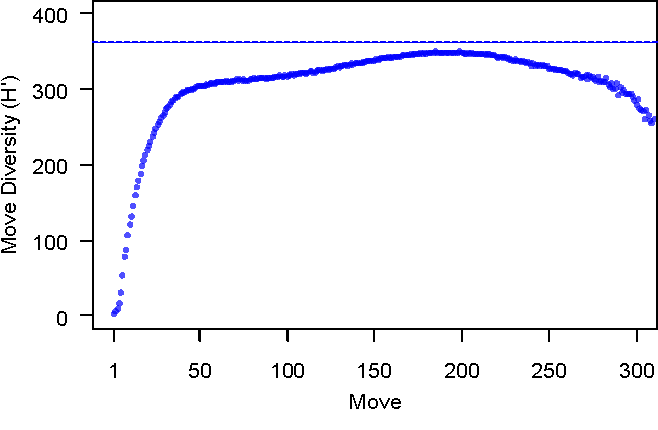
\includegraphics[scale=1.0]{figures/gofirstmove/figShannon.pdf}
\caption{Shannon diversity by game move over the professional database.  For each game move to Move 300, the diversity is calculated via $\exp(-\sum p_j \log(p_j))$, where $p_j$ is the relative frequency of the $j$th variant at that move.  The game eventually approaches a diversity value of 349.23 effective variants at Move 199, indicating that mid-game moves are played at each of 361 intersections on the board with roughly equal frequency across database games.}
\label{fig:Shannon}
\end{center}
\end{figure}

Despite the conservatism of opening play in professional games, novel variations appear regularly and, if widely copied, become new \textit{joseki} in the canon.  Go historian Peter Shotwell writes of the evolution of \textit{joseki}: ``Some are hundreds (or thousands) of years old; others are born, die, and then are reborn again as the style of play changes; still others are yet to be born and patiently wait their turn to be discovered in some flash of ingenuity or desperation.'' \citep{Shotwell2003}

As shown in Figure \ref{fig:M1Freqs}, we can see such dynamics at Move 1 over the latter half of the 20th century.  After a brief enthusiasm for the Threethree in the 1960s, the Fourfour rose to dominance, peaking in 1978 (appearing in 77\% of games played) and again in 1996 (82\% of games played).  As a consequence of these oscillations in the M1 alternatives, we can divide professional play since the 1950s into four major periods (hereafter marked I-IV).  The primary goal of this analysis is to understand why this pattern exists, and what processes are driving its evolution.


\begin{figure}[t]
\begin{center} 
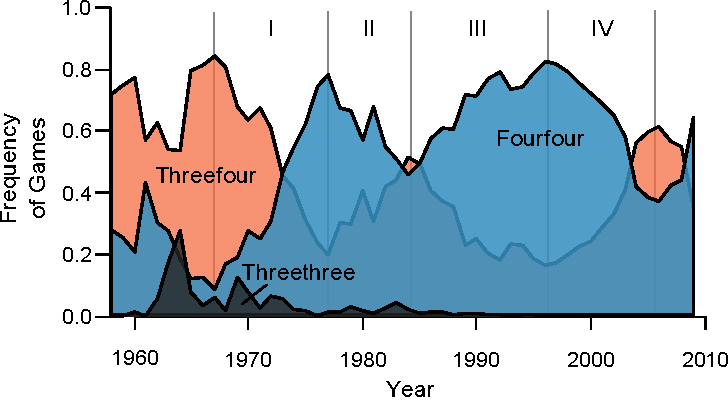
\includegraphics[scale=1.0]{figures/gofirstmove/figM1Freqs.pdf}
\caption{Relative appearance of different variants at Move 1 in the database since 1956.  Because of board symmetry, the M1 Fourfour variant can appear in four different places, and the M1 Threefour variant can appear in eight; the frequencies above take all such congruencies into account.  Based on the cyclic rise and fall of the Fourfour, we can describe four major periods (labeled I-IV) over 20th century professional play.}
\label{fig:M1Freqs}
\end{center}
\end{figure} 
 
 
\section{Cultural Change: Learning versus Demography?}

In general, we consider a cultural trait to \textit{undergo evolution} whenever its distribution within the population changes.  In attempting to explain the oscillatory prevalence of the Move 1 variants over the second half of the 20th century, as described by Figure \ref{fig:M1Freqs}, we can consider a wide variety of underlying evolutionary mechanisms.  Foremost, the enormous amount of study needed to become a professional-level player implies that learning, especially learning from others, is an important source of evolutionary change in Go.
  
Yet, even though standard cultural evolutionary models focus on such social learning, it is important to keep in mind that the distribution of cultural variants in a population can also change due to more ``demographic'' processes.  A change in the age structure, differential migration across the population boundary, or a change in the location of the boundary itself may all bring about cultural change, even though none would be considered ``learning'' or necessarily involve social influence.  If we can establish that the rise of the Fourfour in Period I (1967-1977) is due to, for example, a wave of young Fourfour users joining the professional ranks, then our focus should be the reasons behind this influx, rather than the relatively unimportant learning events taking place within the database.

So, before considering more sophisticated questions about social influence, we have a much more basic and essential task: is the changing prevalence of the Fourfour driven by players altering their behavior (which we'll refer to generically as ``learning''), or is it more due to the demographic replacement of older players as they retire from play with newer players, who enter with a different repertoire of moves?  

The methodology to answer this question is what we call \textit{evolutionary decomposition}, as developed by Coulson and Tuljapurkar \citeyearpar{coulson2008dynamics}, and Beheim and Baldini (in press).  This approach uses individual-level information to exactly partition aggregate change into distinct categories of process.  In Go, there are really only two ways the population can change size: player entry or exit.  Thus, for time periods of arbitrary length, the number of players active in the next period ($N'$) must be related to the number in the current period ($N$) by 
	\[				N' = N + I - E,
\]
where $I$ is the number of players new to the second period, and $E$ the number from the first period absent in the second.  After dividing both sides by $N$, we can express this nondimensionally as 
	\[				G = 1+ i - e.
\]
where $G=N'/N$, $i=I/N$ and $e = E/N$.  If we define player $j$'s ``phenotype'' as $\phi_j$, and assign a ``1'' if they use the Fourfour within their games of a particular time period, and ``0'' if not, we can similarly relate the total number of Fourfour users in successive time periods by
	\[\phi' = \phi + \phi_I + \delta - \phi_E
\]
where $\phi = \sum \phi_j$, $\phi_I$ represents the total number of Fourfour users who have joined the population within the second time period, and $\phi_E$, the total number who have left the population within that period.  The term $\delta$ represents the net balance of those who adopted the Fourfour and those who abandoned it in that time period.  Given these two equations, we can express the change in mean frequency of Fourfour users within the population, $\overline{\phi} = \phi/N$, as
	\[	G \Delta \overline{\phi} = i(\overline{\phi}_I - \overline{\phi}) + c \overline{\delta} - e(\overline{\phi}_E - \overline{\phi}).
\]
Note that $c=1-e$.  Each of the three terms on the right side of the equation describe distinct categories of evolutionary process.  The first term, $i(\overline{\phi}_I - \overline{\phi})$, captures how the mean phenotype among new players alters the mean phenotype of the population, while $e(\overline{\phi}_E - \overline{\phi})$ measures the effect of differential outmigration.  The effect of phenotypic change among those who remain in the population, which here we call ``learning'', is captured by $c \overline{\delta}$. 

Applying this decomposition equation to the game database allows us to see that the Fourfour rose to prominence in Period I almost entirely through learning on the part of professional players, with neglible effects from new players joining the pro community or others leaving it (Figure \ref{fig:PlayerDecomp}).  Here we used two-year periods, but the result holds for one- or five-year periods.  

This result is quite remarkable, considering the major demographic changes taking place in the population.  For 1956, the database used here holds only 105 games, among 18 Black players.  For 2009, 1,354 games are recorded, among 129 unique Black players.  A large part of the explosive growth in the professional Go community can be attributed to changes in nationality; in the 1950s and 1960s, nearly all professionals played in Japan.  In the subsequent decades, professional organizations were established in Korea and China, and by 2009 only about a third of games played are by Japanese players.  Despite these major changes in the size and definition of the population, the decomposition plot indicates that they had very little direct effect on the evolution of M1 variants.  Individual behavioral change is the dominant explanation, and the nature of this change should be the focus of our attention.  


\begin{figure}[t]
\begin{center} 
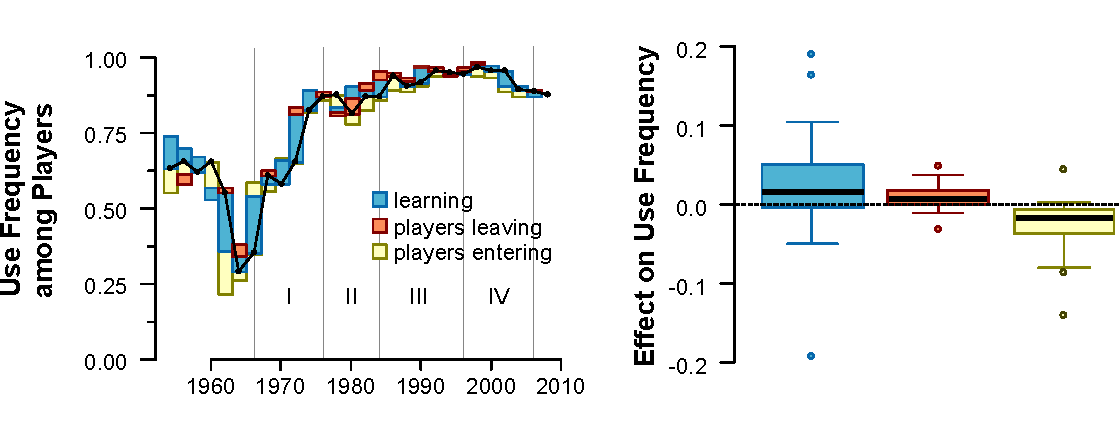
\includegraphics[scale=0.8]{figures/gofirstmove/figPlayerDecomp.pdf}
\caption{Decomposition plot (left) and barplot of decomposition terms (right) for the frequency of use of the Fourfour among players, 1956-2009, using two year periods.  Individual behavioral change (``learning''), rather than population entry and exit, is the dominant explanation of the the rise of the Fourfour during Period I.}
\label{fig:PlayerDecomp}
\end{center}
\end{figure}


% It is naive to think that a single opening move can completely determine victory or defeat, but it is generally understood such moves define the major arc of the game's battles, and are of utmost importance.  

% odd: do the fitted model plots agree with my interpretation of the paraamters??

\section{Are Go Players Social Learners?}

With strong evidence that most of Move 1 evolution in Figure \ref{fig:M1Freqs} can be attributed to professional players altering their behavior (Figure \ref{fig:PlayerDecomp}), we now wish to build a better sense of what motivates such changes.  As strategic actors in a highly competitive environment, Go players are under immense pressure to choose effective moves that help defeat their opponents.  Drawing upon the standard methods in economic and evolutionary theory, we can consider Black's choice at M1 as the result of several plausible models of strategic decision-making \citep{bowles2006microeconomics}.  

(i) \textit{Forward-looking strategic calculation.}  In this model, we imagine rational players who can accurately estimate the future outcomes of particular actions given a set of key input variables, including information about one's general skill compared to that of one's opponent.  Players may choose to try unorthodox or riskier moves against a weaker opponent, who may be less likely to capitalize on their flaws, or when they face a higher handicap.  In such a decision-making model, it is as if the players have complete knowledge of the consequences of using the Fourfour or Threefour variant at Move 1, and simply require the right cues to determine which is best.

(ii) \textit{Recent personal experience.} An obvious problem with forward-looking rationality is that most players cannot realistically determine the value of a move without knowledge of its past use.  Recent experience may show the arrival of a counterstrategy renders a particular move ineffective, and we should expect that players update their valuation of Move 1 variants based on their own past experiences.  

Since records of professional games are widely available (with many of the games taking place in the same locations in Japan and Korea), and the effectiveness of particular choices are difficult to assess from personal experience, we should also expect players to draw upon the information contained in the experiences of others, which we will call ``population knowledge''.  The theoretical literature has concentrated on two simple ways this can be done \citep{boyd1985culture, mcelreath2008beyond}.

(iii) \textit{Success-biased social learning.}  A move that is associated with greater success among other users, regardless of its popularity, may be favored by a focal player.  Similarly, decision-makers may emulate the moves of successful players.  In each case, this strategy rests on a casual association between trait use and the success cue, and so the recent population performance of a particular move should help predict its future use.

(iv) \textit{Frequency-dependent social learning.}  Assuming that players tend to abandon ineffective moves, the prevalence of a move within the Go community itself may be a useful signal of its future performance.  In such situations, we may expect players to simply adopt moves in proportion to their current popularity in the population (``unbiased'' frequency-dependence) or disproportionately favor dominant moves (so-called ``conformity'' bias).  

In both of these cases, players are attending to the experiences of other users, and we should be able to improve our predictions of their behavior by utilizing this information.  Using statistical modeling techniques, we can evaluate how consistent real players are with the idealized models just described, by focusing on three research questions:

\begin{enumerate}
\item Do players employ a particular move coincident with certain features of the match?  If so, what?  The relative ages or recent win records of the players?  The opponent's familiarity with the variant under consideration?
\item Do players tend to respond to their own personal histories with the move?  Are they more likely to play it given past success, or if they have seen it deployed effectively against them in past matches? Could the importance of personal experience with the variant change depending on the focal player's age or recent overall performance?
\item Do players attend to the recent experience of others in the pro community using the move?  Does this interact with the rank or age of the focal player?
\end{enumerate}


\subsection{Methods}

We model the decision to use the Fourfour variant at M1 via a binomial model with a logistic link function of the probability of use, fitted by maximum likelihood in the R programming language.\footnote{In this analysis, we made much use of Ben Bolker's \texttt{bbmle} and Richard McElreath's \texttt{rethinking} packages.}  For each game $j$, we model whether Move 1 was a Fourfour ($y_j=1$) or not ($y_j=0$) via 
\newpage
	\[ y_j \sim \mathrm{Binomial}(1, p_j),
\]
	\[ \mathrm{logit}(p_j) = a + \textbf{xb},
\]
where \textbf{x} is a vector of predictors constructed from other variables in the game database, and \textbf{b}, the vector of corresponding coefficients.

Three major model families were constructed and tested, each embodying one of the above research questions.  The first, ``Match Information'' uses predictors specific to the match; the player's age, win-loss record overall and against this particular opponent, the handicap given to White.  Players who behave according to this model would be forward-looking strategists who can fully anticipate a move's performance and ignore even their own recent experiences, a kind of ``null model'' for learning.  Given that professional players will prepare for a high-profile match by investing a great deal of time reviewing their opponent's games, and that players may be less likely to use a move they know their opponent has commanding mastery of, we also consider the opponent's experience using the Fourfour at Move 1 as a predictor.  

The second model family, ``Personal Knowledge'', includes both a player's recent use of the Fourfour for Move 1, and how often they won games with it, relative to how often they won games without it.  This model corresponds to the hypothesis that players update their views of the move, based on how familiar it is to them and how many games they have won using it.  Finally, ``Population Knowledge'' models use various predictors constructed from the recent population use of the Fourfour, and the population win rate of the Fourfour relative to its alternatives.  These are true social learning models. 

Predictor variables for each game used a retrospective two-year window from the date the game took place, taking the simple average of values for salient games within that period.  Each predictor representing a use frequency was centered on 0.5, a natural point of interpretation for whether a behavior is in the majority.  Predictors for win rate, in contrast, were centered on the average win rate of alternative variants at that game move.  Games in which a predictor was undefined (e.g. a recent win rate for a player's first game) were set to 0 after centering, to drop them out of the model-fitting process.   

Models were fitted and compared in a two-round fashion.  First, within each model family, a variety of models with different combinations of predictor variables were compared using AIC$_c$ and BIC, with top-performing models advancing to the second round.  In the second round, combinations from different model families were constructed and compared.  The top-performing model for each of the three basic model families, as well as the top-performing combination models, are presented in Table \ref{tab:Coeftab}.  


\begin{sidewaystable}[htbp]
  \centering
  \begin{footnotesize}
    \begin{tabular}{lllllll}
	\hline
    \hline
	     & Match & Personal    &  Population   & Match +  & Personal +  & All  \\
          & Information    & Knowledge    &  Knowledge   & Personal   & Population  & Three \\
    \hline
   	Intercept & 0.25 (0.01) & 0.09 (0.02) & 0.08 (0.02) & 0.07 (0.02) & 0.08 (0.02) & 0.02 (0.02) \\
    Personal Win Rate & -0.24 (0.07) &       &       & -0.20 (0.09) &       &  \\
    $\times$ Age & 0.16 (0.05) &       &       & 0.09 (0.07) &       &  \\
    Opponent Use Rate & 1.23 (0.04) &       &       & 0.21 (0.05) &       &  \\
    Handicap (\textit{Komi}) & -0.08 (0.01) &       &       & -0.02 (0.01) &       &  \\
    Per. Use Rate &       & 2.70 (0.11) &       & 2.67 (0.11) & 2.31 (0.11) & 2.30 (0.11) \\
	$\times$ Age  &       &       &       & -0.14 (0.10) &       &  \\
    $\times$ Per. Use Win Rate &       & 0.11 (0.17) &       &       &       &  \\
    (Per. Use Rate)$^2$ &       & 0.28 (0.17) &       & 0.39 (0.17) & 0.29 (0.17) & 0.31 (0.17) \\
    (Per. Use Rate)$^3$ &       & 7.33 (0.61) &       & 6.35 (0.62) & 7.62 (0.62) & 6.79 (0.62) \\
    $\times$ Age &       &       &       & 2.61 (0.53) &       &  2.23 (0.23) \\
    Per. Use Win Rate &       & 0.47 (0.07) &       & 0.39 (0.05) & 0.47 (0.07) & 0.39 (0.05) \\
    (Per. Use Win Rate)$^3$ &       & -0.22 (0.16) &       &       & -0.24 (0.16) &  \\
    Population Use Rate &       &       & 3.06 (0.17) &       & 0.27 (0.19) & 0.32 (0.19) \\
    $\times$ Pop. Use Win Rate &       &       & 9.02 (1.68) &       & 11.04 (1.88) & 9.34 (1.74) \\
    $\times$ Age &       &       &       &       &       & -0.27 (0.07) \\
    $\times$ Per. Use Win Rate &       &       &       &       &       & -1.19 (0.46) \\
    (Pop. Use Rate)$^2$ &       &       & -0.81 (0.43) &       & -1.20 (0.49) &  \\
    (Pop. Use Rate)$^3$ &       &       & 11.95 (2.14) &       & 9.34 (2.36) & 10.48 (2.28) \\
    Pop. Use Win Rate &       &       & 2.30 (0.33) &       & 2.09 (0.37) & 1.82 (0.36) \\
    (Pop. Use Win Rate)$^2$ &       &       & -8.41 (4.28) &       & -10.04 (4.89) &  \\
    \hline
    Validation Error & 38.94 (0.82)  & 26.81 (0.65)  & 34.00 (0.68) & 26.72 (0.66) & 26.63 (0.65) & 26.70 (0.74) \\
    Neg. log Likelihoods & 22586.25 & 18111.59 & 21121.34 & 18054.59 & 17982.01 & 17936.31 \\
    AIC$_c$ weight & $<$0.001  & $<$0.001     & $<$0.001     & $<$0.001     & $<$0.001     &  .99 \\
    \hline
    \end{tabular}%
	\caption{Estimates and standard errors for the top model in each of the three basic model families, plus three combination families.  Both AIC$_c$ and BIC nominate the top model in the ``All Three'' family unequivocally, though the only surviving predictor variables in this model from ``Match Information'' are age interactions.  Model comparison was also done through 10-fold cross-validation, resulting in logistic error rates for each model lower than the baseline error of 41.1\%.}
	\label{tab:Coeftab}%
    \end{footnotesize}
\end{sidewaystable}%


\subsection{Results}

Unsurprisingly, a player's recent use of the Fourfour at M1 strongly predicts their current use: using the ``divide by four'' rule to interpret logistic regression coefficients, a 10 percent difference in past use corresponds to, at most, a 6 percentage point difference in the probability Black will deploy the Fourfour in the current game.  Past personal success with the Fourfour is also predictive, but not as much; an otherwise average player who wins 60\% of their Fourfour games will be about one percentage point more likely to use the Fourfour than a similar player who wins 50\% of recent Fourfour games.  

By itself, the population's recent use of the Fourfour is not as predictive of Black's behavior on M1.  When the Fourfour appears in 60\% of all recent games, the expected probability of use by an average player is only 0.52, compared to 0.50 when the Fourfour appears in half of recent games (Figure \ref{fig:mABCplots}).  However, it is a mistake to think population use is unimportant; it has a large interaction with the Fourfour's relative win rate in the population.  If the Fourfour is at 60\% use and its performance is 10 percentage points higher than that of its rival, the Threefour, the expected probability of use is now 0.58, slightly larger than an equivalent situation for personal use and performance.  

This interaction between popularity and performance in recent games is in fact the largest effect in the top model, strong evidence towards the view Go players are social learners.  But the interaction implies this social learning is \textit{strategic}.  Players are insensitive to a move's popularity when it performs about as well as its rivals, but appear to be quite responsive to the popularity of a high-performing move (Figure \ref{fig:mABCplots}). 

Interestingly, age diminishes the effect of population knowledge but strengthens that of personal knowledge.  In the above scenario (60\% pop. use and $+$10\% pop. win rate) and under the ``All Three'' model, an otherwise average professional in their late teens will use the Fourfour with probability 0.59, while a similar player in his early sixties will only use it with probability 0.56.  In contrast, age strengths the predictive importance of one's personal past use slightly, about half a percentage point for a difference in age of ten years.  

Taken together, this could reflect the behavioral consequences of aging; older players are less willing to change their behavior and less sensitive to trends in the population.  However, older players also tend to be self-selected by performance and rank, so this could alternatively reflect a difference in underlying skill that is present throughout their careers.

Several predictors that were included in each of the early rounds never made it to reported models, including the number of matches played against the current opponent, how successful that opponent has been with the Fourfour recently, the proportion of those matches won, the number of matches in which the Fourfour was used against the focal player (playing as White).  Notably, the population size (i.e. number of active players) itself was predictively irrelevant, both as a main effect and in regulating the importance of population use rate and population use win rate via interactions.

Also noteworthy is that almost all of the ``match-specific'' predictors were excluded in the best-performing model.  Opponent's use of the Fourfour, a strong positive predictor in the ``Match Only'' family, drops out completely once personal knowledge and population knowledge are included.

\begin{figure}[tp]
\begin{center} 
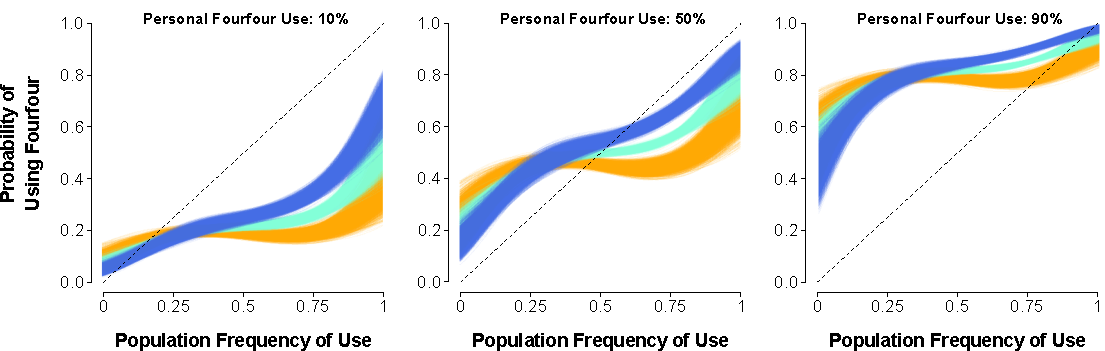
\includegraphics[scale=0.8]{figures/gofirstmove/figmABCplots.pdf}
\caption{Predicted probability of using the Fourfour from the top-performing model, ``All Three'', with uncertainty described by sampling from the joint posterior 5,000 times.  In each panel, the model predicts a response to differences in population use of the Fourfour at three levels of population performance: 10 percentage points better than alternatives (blue), 10 percentage points below alternatives (orange) and performance equivalence (aquamarine).  Players are predicted to be more insensitive to population frequency values when the Fourfour performs about the same as its alternatives at M1.}
\label{fig:mABCplots}
\end{center}
\end{figure}

As demonstrated in Figure \ref{fig:FourfourPredicted}, the ``All Three'' model provides an excellent reconstruction of the observed periodic trajectory of the Fourfour.  Ignoring population knowledge misses the major swings at the zenith and nadir of each cycle, while ignoring personal knowledge produces wide prediction intervals.  Additionally, our top model from the``All Three'' family has an error rate of 26.5\% on the observed data, down from the baseline error rate of 43\%.  Similar values were recovered through ten-fold cross-validation, in which the fitted model makes predictions on new data it has never seen (Table \ref{tab:Coeftab}).
			
% It spread in large part because other players were winning games with it.  This is a broad sketch of a deep story, as the opening move is not in isolation, but associated with.  The win rate with the move seems to indicate that innovative openings using the move allowed it to take off and succeed.  

% So what was difference about 1967 and 1977?  Few people used the move, but those that did saw a remarkable increase in performance, which drove its popularity.  The majority of this effect was social - people saw others doing well using the move.  At its peak in 1977, the interaction between use and wining resulted in a very large effect indeed.  It really was winning more.  Once this trend reversed in the early 80s, the Fourfour waned.


\begin{figure}[t]
\begin{center} 
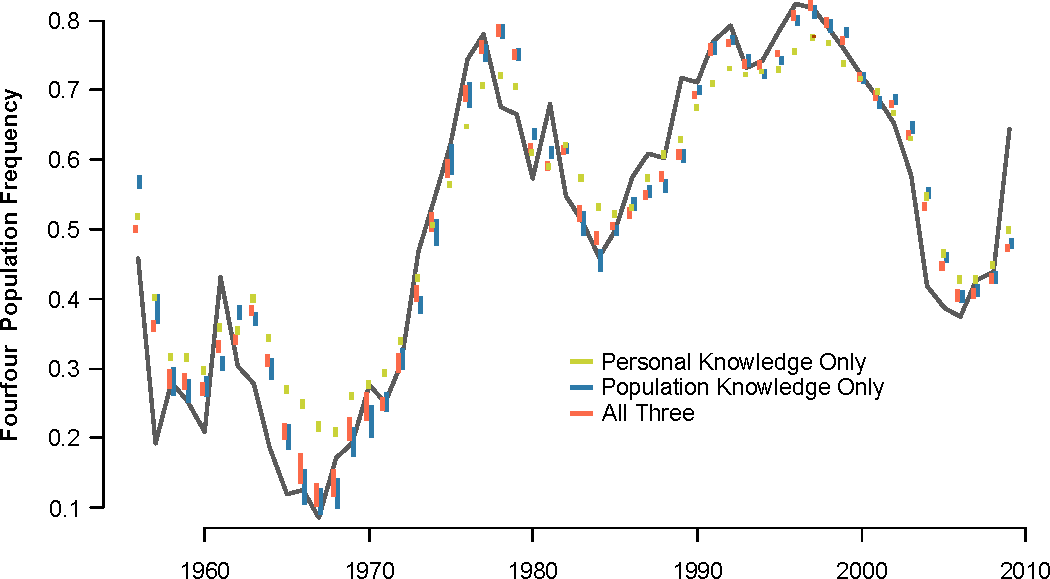
\includegraphics[scale=0.7]{figures/gofirstmove/figFourfourPredicted.pdf}
\caption{The observed and predicted prevalence of the Fourfour variant over time, with each bar spanning the 95\% prediction interval around the maximum likelihood estimate.  Green is the trajectory predicted by the ``Personal Knowledge'' model.  It has a lower logistic error rate (27\%) but does not track population trends closely.  The ``Population Knowledge'' population model (blue) tracks the observed trends more accurately but has wide prediction intervals.  The full model, ``All Three'' (red) is more accurate than personal history alone, since it includes the recent behavior of others, but it is more precise than population history alone.}
\label{fig:FourfourPredicted}	
\end{center}
\end{figure}



\section{Arms Races and Innovation Cycles} \label{sec:Arms}

% cite Boyd and Richerson 1992 on "how microevolutionary processes give rise to history" - the key is the relationship between historical events and process summaries requires you talk about both
 
To summarize, the above has established that (1) most of the change in the prevalence of the Fourfour variant at Move 1 over time is due to learning, rather than demographic changes, and (2) individuals appear to judge a particular variant using social knowledge, namely its overall popularity and relative success.

Despite the fact that the first move of the game hundreds of moves long does not guarantee victory or defeat, how well a particular M1 variant does relative to alternatives within the population is a robust predictor of use.  As indicated by the ``All Three'' model, the Fourfour enjoyed an anomalously large win rate in Period I, during which it proliferated rapidly in the professional community (Figure \ref{fig:M1FreqsWins}).  Conversely, when it declines in Period II, its win rate is consistently below that of its rival variant, the Threefour.

This connection to performance aids our ability to explain the historical record, but we cannot yet say \textit{why} this performance difference exists in the first place, and why the Fourfour did relatively well during Period I and III, but poorly in Period II and IV.  Without the knowledge and skills of a professional player, this may be impossible to fully answer.  However, it is possible to trace the sucess of the Fourfour of 20th century play to particular individuals and events.  From this evidence, it appears that the waxing and waining success of the Fourfour appears to stem from an ongoing crucible of innovation and counterinnovation.

\subsection{Period I: Initial Rise, 1967-1977}

 \begin{figure}[t]
\begin{center} 
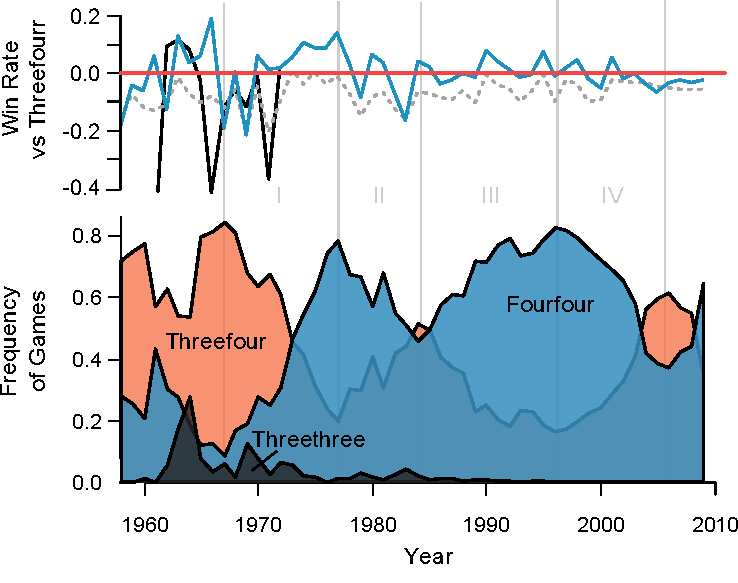
\includegraphics[scale=1.0]{figures/gofirstmove/figM1FreqsWins.pdf}
\caption{The ebb and flow of the three major first move variants, with proportion of games won.  The Fourfour's rise and fall closely tracks with its relative performance (blue line) since 1967.  Similarly, the Threethree's brief efflorescence and extinction closely match its relative win rate (black line).  Because of its initial dominance, all win rates are expressed relative to the Threefour's (red line), and the dotted gray line indicates the location of the 50\% (break-even) point.}
\label{fig:M1FreqsWins}
\end{center}
\end{figure}
 
\begin{figure}[t]
\begin{center} 
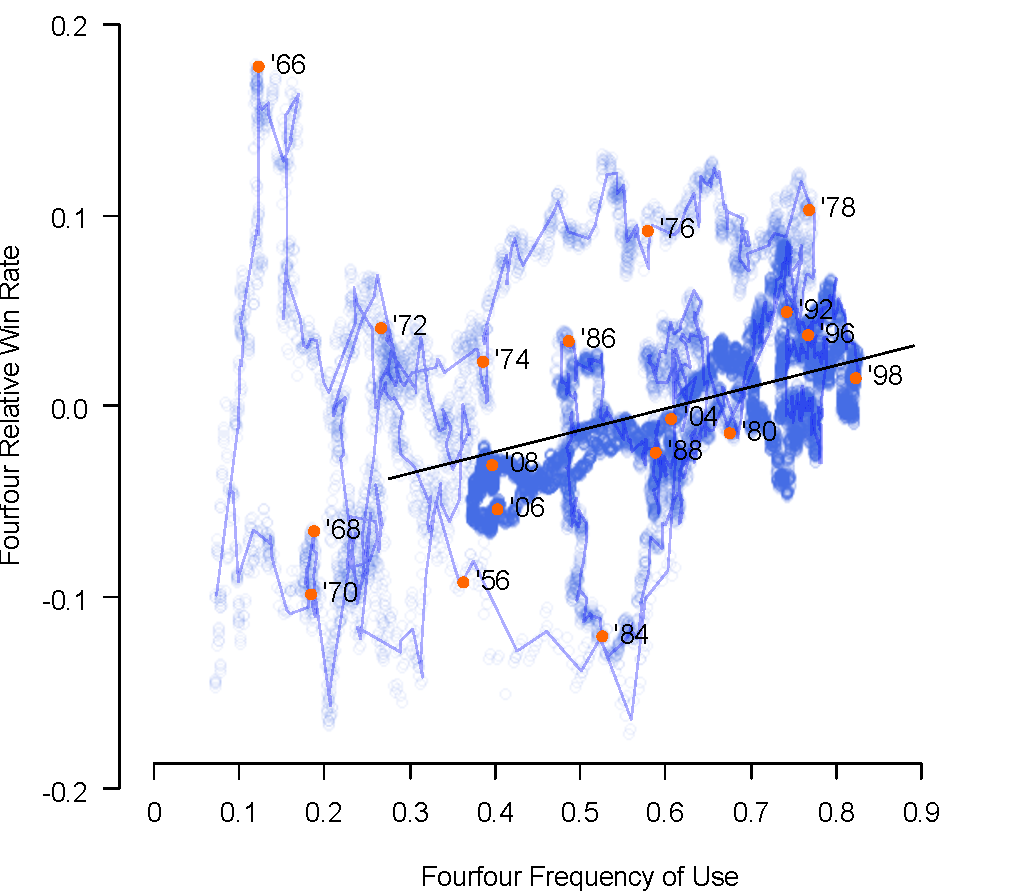
\includegraphics[scale=0.75]{figures/gofirstmove/figSuccessCycle.pdf}
\caption{Recent use of the Fourfour plotted against its recent win rate (r=0.45, with fitted OLS line).  Since its rapid diffusion in the 1970s, the Fourfour's prevalence at M1 has settled into a regular cycle between popularity/success (1978, 1996) and unpopularity/underperformance (1984, 2006).  If this pattern holds, the next peak in popularity should be sometime around 2016.}
\label{fig:SuccessCycle}
\end{center}
\end{figure}

\begin{figure}[t]
\begin{center} 
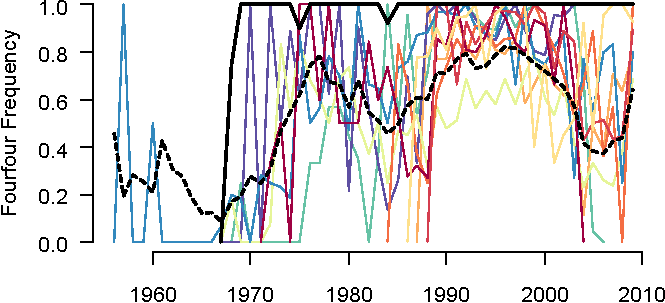
\includegraphics[scale=1.0]{figures/gofirstmove/figPersonalFourfour.pdf}
\caption{Percent of games using Fourfour by population (dashed black line) and by player (colored lines) for the ten most prolific users of the Fourfour.  Takemiya Masaki, who almost always uses the Fourfour, appears as a solid black line.}
\label{fig:PersonalFourfour}
\end{center}
\end{figure}
 
Among Go professionals, one player seems most responsible for the rise of the Fourfour in the 1960s and 1970s: Takemiya Masaki.  Beginning his professional career at the age of 14, Takemiya arrived at the Fourfour's nadir in 1965, and in the database he began using it in 1968.  Takemiya's loose, center-oriented playing style, widely known as ``Cosmic Go'', involves the Fourfour at Move 1 almost exclusively; among his 520 games as Black in the database, only 6 do not start with the Fourfour at M1\footnote{Of these, four are Threefour, one is Threethree, and one is Fourfive.}.  Takemiya's use of the Fourfour coincides with the beginning of Period I and its proliferation within the broader Go community (Figure \ref{fig:PersonalFourfour}).  During this time, his personal performance as Black (61.8\%) also exceeded the average win rate for Black (59\%).  

His influence in starting this trend is apparently a known fact among professionals themselves.  In a 1994 interview with the British Go Journal, Korean master player Seo Pong-su noted that, ``Before him [Takemiya], Korean amateurs and professionals used to avoid the 4-4 point; now this is the most popular opening.'' and attributed Takemiya's innovative play to his greater willingness to research vague, risky moves \citep{Finch1994}.	    

It is interesting to note that the Fourfour was used at M1 before the 1960s, and Takemiya is obviously not its inventor.  However, its success and rapid diffusion is consistent with the hypothesis that Takemiya and his successors hit upon a \textit{new way to use} the Fourfour within the subsequent moves of the game, and this development has had a major effect on strategic landscape of professional Go.

\subsection{Period II: Counterinnovation and Decline, 1977-1984}

 \begin{figure}[t]
\begin{center} 
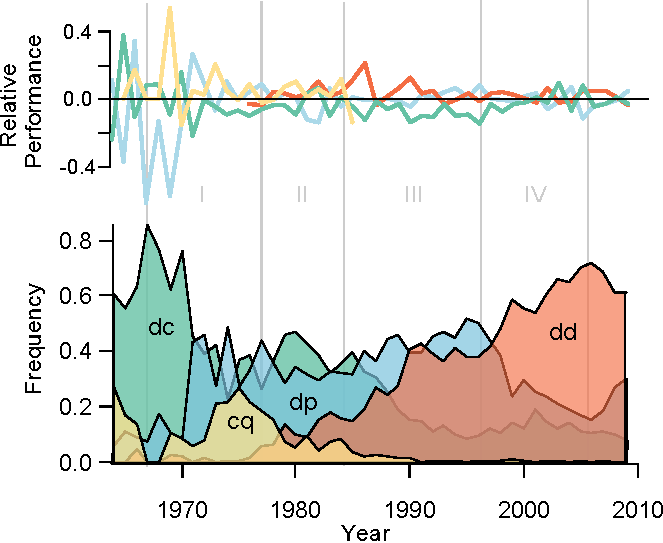
\includegraphics[scale=1.0]{figures/gofirstmove/figM2FreqsWins.pdf}
\caption{Frequency and performance for four major M2 responses to the Fourfour.  Performance for each is calculated as the win rate subtracting the average win rate of alternatives.  As at M1, a variants's frequency closely tracks its relative performance.}
\label{fig:M2FreqsWins}
\end{center}
\end{figure}

Subsequent to Takemiya's arrival, the success of the Fourfour appears to have prompted an innovation race in White's Move 2 response.  Before 1970, White's response to the  Fourfour was almost always a Threefour on an adjacent corner.  If we imagine the M1 Fourfour is played in the upper right quadrant (SGF coordinate pd), nearly 80\% of the time the M2 response in the late 1960s was coordinate dc (Figure \ref{fig:M2FreqsWins}).  By 1977, at the Fourfour's first peak, the M2 dc variant appeared only about 30\% of the time.  During that time, M2 variants dp, cq and dd all became established moves in rapid sequence.  As measured by the proportion of games White won, cq and then dd both consistently outperformed dp during the early 1980s, blunting the Fourfour's effectiveness and anticipating its decline in use.

As with the Fourfour variant at M1, the dd response appeared suddenly, and its early successes can be traced to a single individual, Kudo Norio.  Kudo began using the move in 1977 and won 3 of the 4 games he tried it in (Table \ref{tab:M2dd}).  The next year, he won 4 of 6 attempts, including one against Takemiya (reproduced as Figure \ref{fig:Kifu}).  By 1981, over a dozen professionals were using this M2 variant, and over the next 30 years dd would steadily rise in the professional community to become the dominant response to the M1 Fourfour, followed by dp (Figure \ref{fig:M2FreqsWins}).  It is interesting to note that both of these responses are, by board position, also Fourfours.  

\begin{sidewaystable}[htbp]
  \centering
  \begin{footnotesize}
    \begin{tabular}{rlr|rlr|rlr}
    \hline
	\hline
    1975  & Hasmimoto Utaro & 1 of 1 & 1979  & Cho Chikun & 1 of 2 & 1981  & Cho Chikun & 0 of 1 \\
    1974  & Kato Masao & 0 of 1 &       & Ishida Yoshio & 1 of 6 &       & Fujisawa Hideyuki & 2 of 3 \\
    1976  & Hasmimoto Utaro & 1 of 1 &       & Kobayashi Koichi & 0 of 1 &       & Ishida Yoshio & 1 of 2 \\
          & Takagi Shoichi & 0 of 1 &       & Kudo Norio & 2 of 3 &       & Ishigure Ikuro & 0 of 1 \\
          & Takemiya Masaki  & 0 of 1 &       & Sakata Eio & 5 of 9 &       & Kataoka Satoshi & 1 of 1 \\
    1977  & Cho Chikun & 0 of 3 &       & Takemiya Masaki  & 1 of 2 &       & Ni Linqiang & 0 of 1 \\
          & Hashimoto Utaro & 0 of 1 &       & Ushinohama Satsuo & 2 of 2 &       & Nie Weiping  & 1 of 1 \\
          & Iwata Tatsuaki & 0 of 1 & 1980  & Fujisawa Hideyuki & 2 of 2 &       & Sakata Eio & 2 of 4 \\
          & \textbf{Kudo Norio} & \textbf{3 of 4} &       & Hashimoto Utaro & 0 of 1 &       & Shinkai Hiroko & 0 of 1 \\
          & Takemiya Masaki  & 0 of 3 &       & Ishida Yoshio & 0 of 2 &       & Sugiuchi Masao & 1 of 1 \\
    1978  & Fujisawa Hideyuki & 0 of 1 &       & Kudo Norio & 1 of 1 &       & Takagi Shoichi & 0 of 1 \\
          & Hisai Keishi & 1 of 2 &       & Otake Hideo & 0 of 1 &       & Takemiya Masaki  & 0 of 1 \\
          & \textbf{Kudo Norio} & \textbf{4 of 6} &       & Sakata Eio & 2 of 8 &       & Yamashiro Hiroshi & 1 of 2 \\
          & Magari Reiki & 0 of 1 &       & Takagi Shoichi & 0 of 1 &       &       &  \\
          & Sakata Eio & 0 of 1 &       & Takemiya Masaki  & 1 of 1 &       &       &  \\
          & Ushinohama Satsuo & 0 of 1 &       &       &       &       &       &  \\
    \hline
    \end{tabular}%
	\caption{List of players using the M2 dd move in response to the M1 Fourfour, 1975-1981, with the number of games won out of the number attempted.  Kudo Norio's remarkable success in 1977 and 1978 anticipates the dd variant's proliferation (Figure \ref{fig:M2FreqsWins}).  One of Kudo's winning 1978 games, against the modern pioneer of the Fourfour, is reprinted as Figure \ref{fig:Kifu}.}
	\label{tab:M2dd}%
	\end{footnotesize}
\end{sidewaystable}%



\section{Discussion}

Though only a preliminary treatment of a very rich dataset, the above results demonstrate how a socially-transmitted cultural pattern of behavior - the move variants at M1 and M2 in the game of Go - undergo evolutionary change.  From the above evidence, it seems that the average professional player uses both personal knowledge and social knowledge to decide which move to use in a particular game.  Using evolutionary decomposition, we can show that, despite major growth in the professional community and addition of players from China and Korea, the population dynamics of opening moves is driven by learning on the part of active players, rather than demographic effects from influx of younger players or outflux of older players.  A player's recent use of a move at M1 effectively predicts their future behavior, indicating players update their play based on past experiences.  This association increases with age; older players are better predicted by their play in the last two years than younger players.  Personal win rate using the variant also aids in prediction, but this effect is not as strong as a player's past use. 

We also have evidence that players use population knowledge; a professional's behavior at M1 is strongly predicted by the recent population performance of particular variants.  The population frequency of an M1 variant is also predictive, but only when that variant is, on the average, winning more (or fewer) games than its rivals.  The conditional importance of the Fourfour's popularity seems to indicate that players use the frequency information strategically, since the theoretical advantages of frequency-dependent learning strategies come from an association between popularity and performance.  

Given these results, it should be no surprise that the Fourfour's prevalence is strongly associated with its recent performance since the 1960s.  By looking at particular games, we can also see how the breakaway success of the Fourfour variant at M1 was followed by a period of innovation and diversity in more effective M2 responses.  Taken together, this evidence all seems to indicate an ongoing evolutionary arms race taking place within the opening moves of professional Go.  

Although we can do much to reconstruct and explore the historical record, several important questions remain outstanding.  First, we do not know the nature of the observed success bias.  We can see that relative performance of the Fourfour versus the Threefour consistently improves our predictions of which one a particular player will use.  This seems to indicate players focus on how well a move does, but it is equally possible, however, that successful \textit{players} rather than successful variants are what are emulated.  

This is not captured by crude measures like population use frequency, and is indicative of a larger problem: establishing exactly who players are learning from.  The statistical models above treat the general population as an equally-connected, homogenous pool.  Real social influence in this situation undoubtedly involves a variety of complex social relationships between unique personalities.  The nature of these influences may be better captured by network-based approaches that allow for heterogeneous interconnections between players.  It may be possible to use information about players' nationalities or recent matches to develop measures of social proximity, allowing the detection of theoretical effects like conformist learning or prestige.

Another problem is the nature of innovation in Fourfour play.  Even if Takemiya's ``Cosmic'' opening style was the catalyst for the Fourfour's rise in Period I, as the evidence above seems to indicate, we do not know if other adopters were using it in the same way.  The observed pattern could be, for example, due to Takemiya's early successes in 1968-1970 encouraging other professionals to revisit the Fourfour and develop their own innovative applications, rather than emulate his.  

Finally, even if players really are using a combination of individual and population knowledge, we should consider the possibility that this offers no real strategic advantage.  A well-understood problem with success bias is that it aims to exploit an association between use and performance, but can lead to the proliferation of neutral or even deleterious practices if that association is not causal.  The dynamics described above would exist even if the first move has little impact on the subsequent game, provided only that players \textit{think} it does. 

There are many more possible avenues of exploration in this very rich dataset.  Venturing beyond Move 2, we can study the diffusion of particular \textit{joseki} patterns, the importance of particular high-status individuals (like the Go Seigen interview described above) or, indirectly, the diffusion of particular Go proverbs within profesisonal play.  The scope of study can also be expanded; large archives of professional games go back at least several hundred years, and tens of thousands of amateur games are available online, to say nothing of similar archives available for other games like chess.  

In any case, the statistical and theoretical tools employed above can be used to expand our understanding of cultural dynamics.  The above results hopefully demonstrate the value of taking a quantitative, Darwinian point of view towards cultural change.  As in evolutionary ecology, we can use the results of high-resolution datasets to help understand, indirectly, historical dynamics for which little data remains and variants are harder to define.  Indeed, we feel that the theroetical and empirical evidence is so overwhelming that the key question is not ``whether'' culture evolves, but rather which day-to-day learning and demographic processes brought about the particular patterns of cultural diversity we see in human history.  






% This innovation can also be correlated to the size of the professional community as well.  To put it simply, more individuals means more innovation and faster arms race dynamics.  










